
\newcommand*{\xMin}{0}%
\newcommand*{\xMax}{12}%
\newcommand*{\xStep}{1}%
\newcommand*{\xStepp}{1.5}%
\newcommand*{\nStep}{3}
\newcommand*{\nStepp}{2}
\newcommand*{\yMin}{0}%
\newcommand*{\yMax}{1}%

\newcommand\markcell[3] {
  %\fill[white,draw=black] (#2*\xStep,\xStep*\nStep-#1*\xStep) -- (#2*\xStep+\xStep,\xStep*\nStep-#1*\xStep) -- (#2*\xStep+\xStep,\xStep*\nStep-#1*\xStep-\xStep) -- (#2*\xStep,\xStep*\nStep-#1*\xStep-\xStep) -- cycle;
  \node[anchor=center] at (#2*\xStep+0.5*\xStep,\xStep*\nStep-#1*\xStep-0.5*\xStep) {#3};
  }

\newcommand\markcelll[3] {
  %\fill[white,draw=black] (\xStep*\nStep+#2*\xStepp,\xStepp*\nStepp-#1*\xStepp) -- (\xStep*\nStep+#2*\xStepp+\xStepp,\xStepp*\nStepp-#1*\xStepp) -- (\xStep*\nStep+#2*\xStepp+\xStepp,\xStepp*\nStepp-#1*\xStepp-\xStepp) -- (\xStep*\nStep+#2*\xStepp,\xStepp*\nStepp-#1*\xStepp-\xStepp) -- cycle;
  \node[anchor=center] at (\xStep*\nStep+#2*\xStepp+0.5*\xStepp,\xStepp*\nStepp-#1*\xStepp-0.5*\xStepp) {#3};
  }

\newcommand\markcelllorange[3] {
  \fill[orange,draw=black] (\xStep*\nStep+#2*\xStepp,\xStepp*\nStepp-#1*\xStepp) -- (\xStep*\nStep+#2*\xStepp+\xStepp,\xStepp*\nStepp-#1*\xStepp) -- (\xStep*\nStep+#2*\xStepp+\xStepp,\xStepp*\nStepp-#1*\xStepp-\xStepp) -- (\xStep*\nStep+#2*\xStepp,\xStepp*\nStepp-#1*\xStepp-\xStepp) -- cycle;
  \node[anchor=center] at (\xStep*\nStep+#2*\xStepp+0.5*\xStepp,\xStepp*\nStepp-#1*\xStepp-0.5*\xStepp) {#3};
  }

  \newcommand\markcel[2] {
    %\fill[orange,draw=black] (0,-#1*0.25*\xStep) -- (0.25*\xStep,-#1*0.25*\xStep) -- (0.25*\xStep,-#1*0.25*\xStep-0.25*\xStep) -- (0,-#1*0.25*\xStep-0.25*\xStep) -- cycle;
    \node[anchor=center] at (-0.25*\xStep,-#1*0.25*\xStep-0.125*\xStep) {\footnotesize #2};
  }

  \newcommand\markcelorange[2] {
    \fill[orange,draw=black] (0,-#1*0.25*\xStep) -- (0.25*\xStep,-#1*0.25*\xStep) -- (0.25*\xStep,-#1*0.25*\xStep-0.25*\xStep) -- (0,-#1*0.25*\xStep-0.25*\xStep) -- cycle;
    \node[anchor=center] at (-0.25*\xStep,-#1*0.25*\xStep-0.125*\xStep) {\footnotesize #2};
  }


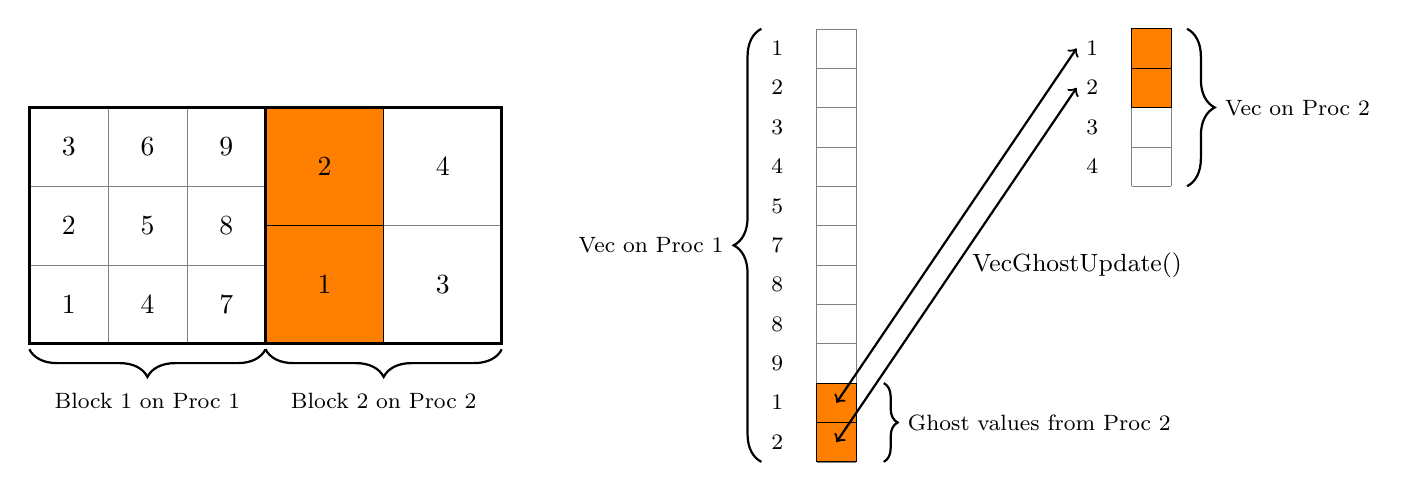
\begin{tikzpicture}


    \foreach \j in {0,...,\nStep} {
        \draw [very thin,gray] (0,\j*\xStep) -- (\xStep*\nStep,\j*\xStep)  ;
        \draw [very thin,gray] (\j*\xStep,0) -- (\j*\xStep,\xStep*\nStep)  ;
    }
    \markcell{0}{0}{3};
    \markcell{0}{1}{6};
    \markcell{0}{2}{9};

    \markcell{1}{0}{2};
    \markcell{1}{1}{5};
    \markcell{1}{2}{8};

    \markcell{2}{0}{1};
    \markcell{2}{1}{4};
    \markcell{2}{2}{7};

    \foreach \j in {0,...,\nStepp} {
        \draw [very thin,gray] (\xStep*\nStep,\j*\xStepp) -- (\xStep*\nStep+\xStepp*\nStepp,\j*\xStepp)  ;
        \draw [very thin,gray] (\xStep*\nStep+\j*\xStepp,0) -- (\xStep*\nStep+\j*\xStepp,\xStepp*\nStepp)  ;
    }

    \markcelllorange{0}{0}{2};
    \markcelll{0}{1}{4};

    \markcelllorange{1}{0}{1};
    \markcelll{1}{1}{3};

    \draw[very thick] (0,0) rectangle (\xStep*\nStep,\xStep*\nStep);
    \draw[very thick]  (\xStep*\nStep,0) rectangle (\xStep*\nStep+\xStepp*\nStepp,\xStepp*\nStepp) ;

    \begin{scope}[shift={(10,4)},scale=2]
    \foreach \j in {0,...,10} {
        \draw [very thin,gray] (0,-0.25*\j*\xStep) -- (0.25*\xStep,-0.25*\j*\xStep)  ;
        \draw [very thin,gray] (0,-0.25*\j*\xStep) -- (0,-0.25*\j*\xStep-0.25*\xStep)  ;
        \draw [very thin,gray] (0.25*\xStep,-0.25*\j*\xStep) -- (0.25*\xStep,-0.25*\j*\xStep-0.25*\xStep)  ;
    }
    \draw [very thin,gray] (0,-0.25*11*\xStep) -- (0.25*\xStep,-0.25*11*\xStep)  ;
    \markcel{0}{1};
    \markcel{1}{2};
    \markcel{2}{3};
    \markcel{3}{4};
    \markcel{4}{5};
    \markcel{5}{7};
    \markcel{6}{8};
    \markcel{7}{8};
    \markcel{8}{9};
    \markcelorange{9}{1};
    \markcelorange{10}{2};
    \draw[<->,thick,bend right,bend angle=40]  (0.125*\xStep,-9*0.25*\xStep-0.125*\xStep) -- (2-0.35*\xStep,-0*0.25*\xStep-0.125*\xStep);
    \draw[<->,thick]  (0.125*\xStep,-10*0.25*\xStep-0.125*\xStep) -- (2-0.35*\xStep,-1*0.25*\xStep-0.125*\xStep) node [midway,right,xshift=2pt] {\small VecGhostUpdate()};

    \draw [thick,decorate,decoration={brace,amplitude=10pt},xshift=-10pt]
    (0.0,-2.75) -- (0.0,0.0) node [black,midway,left,xshift=-10pt] 
    {\footnotesize Vec on Proc $1$};

    \draw [thick,decorate,decoration={brace,amplitude=5pt},xshift=5pt]
    (0.25,-2.25) -- (0.25,-2.75) node [black,midway,right,xshift=5pt] 
    {\footnotesize Ghost values from Proc $2$};


   \end{scope}

    \begin{scope}[shift={(14,4)},scale=2]
    \foreach \j in {0,...,3} {
        \draw [very thin,gray] (0,-0.25*\j*\xStep) -- (0.25*\xStep,-0.25*\j*\xStep)  ;
        \draw [very thin,gray] (0,-0.25*\j*\xStep) -- (0,-0.25*\j*\xStep-0.25*\xStep)  ;
        \draw [very thin,gray] (0.25*\xStep,-0.25*\j*\xStep) -- (0.25*\xStep,-0.25*\j*\xStep-0.25*\xStep)  ;
    }
    \draw [very thin,gray] (0,-0.25*4*\xStep) -- (0.25*\xStep,-0.25*4*\xStep)  ;
    \markcelorange{0}{1};
    \markcelorange{1}{2};
    \markcel{2}{3};
    \markcel{3}{4};

    \draw [thick,decorate,decoration={brace,amplitude=10pt},xshift=10pt]
    (0.0,0.0) -- (0.0,-1) node [black,midway,right,xshift=10pt] 
    {\footnotesize Vec on Proc $2$};
   \end{scope}

\draw [thick,decorate,decoration={brace,amplitude=10pt},yshift=-2pt]
(3.0,0.0) -- (0.0,0.0) node [black,midway,below,yshift=-12pt] 
{\footnotesize Block $1$ on Proc $1$};

\draw [thick,decorate,decoration={brace,amplitude=10pt},yshift=-2pt]
(6.0,0.0) -- (3.0,0.0) node [black,midway,below,yshift=-12pt] 
{\footnotesize Block $2$ on Proc $2$};

\end{tikzpicture}
